\part{Opis matematyczny modelu}

\chapter{Gen~6 w jednym miejscu: pełny opis matematyczny}\label{rozdz:opis}

\section{Po co jeszcze jeden rozdział?}

W poprzednich rozdziałach model powstawał kawałek po kawałku. Teraz zbieramy go w całość: jedna lista oznaczeń, jedno złożenie funkcji, jeden wzór na liczbę parametrów, jedna tabela kształtów. Rozdział można czytać samodzielnie jako
\emph{specyfikację} modelu; wszystkie wzory były już wyprowadzone, a odsyłacze wskazują, gdzie.

Po tym rozdziale umiesz: (i)~zapisać Gen~6 jako złożenie funkcji z kształtami, (ii)~policzyć liczbę parametrów dla dowolnych hiperparametrów, (iii)~przeprowadzić nagranie przez cały model od fali do listy nut, (iv)~odesłać każdy element do rozdziału, w którym jest uzasadniony.

\section{Oznaczenia}

\begin{table}[ht]
\centering\small
\begin{tabular}{@{}llp{6.1cm}@{}}
\toprule
symbol & wartość & znaczenie\\
\midrule
$f_s$ & $11\,025\Hz$ & częstotliwość próbkowania po zmianie\\
$T$ & --- & liczba klatek ($T=\lfloor(N-4096)/256\rfloor+1$)\\
$C,\ P,\ S$ & $9,\ 159,\ 53$ & kanały HCQT, biny wysokości, półtony ($P=3S$)\\
$H,\ D$ & $48,\ 64$ & szerokość części konwolucyjnej i kontekstowej\\
$n_h,\ d_h$ & $4,\ 16$ & głowice uwagi i ich wymiar ($D=n_hd_h$)\\
$W$ & $43$ & półokno uwagi w czasie (klatki)\\
$K=(k_1,\dots,k_7)$ & $(-36,0,36,57,72,84,93)$ & przesunięcia alikwotów w binach\\
$d_1,d_2,d_3$ & $1,2,4$ & dylatacje czasowe bloków\\
$o_1,\dots,o_6$ & $64,59,55,50,45,40$ & struny puste (od najcieńszej)\\
$\theta$ & $249\,219$ liczb & wszystkie parametry sieci\\
\bottomrule
\end{tabular}
\caption{Stałe i hiperparametry Gen~6 (\texttt{gen6\_kaggle.json}).}
\label{tab:oznaczenia}
\end{table}

\section{Model jako złożenie}

Nagranie $x\in\R^N$ (po zmianie próbkowania do $f_s$) przechodzi przez osiem etapów. Wszystkie znaki zostały zdefiniowane wcześniej: $\GELU$ (def.~\ref{def:gelu}), $\LN$ (def.~\ref{def:ln}), $\Drop$ (def.~\ref{def:dropout}), $\shift$ (def.~\ref{def:shift}), $\Conv$ i $\DW$ (def.~\ref{def:konwolucja}).

\begin{definicja}[Model Gen~6]\label{def:gen6}
\textbf{(0) Cechy.} $X=\mathrm{HCQT}(x)\in\R^{C\times T\times P}$ (def.~\ref{def:hcqt}, \ref{def:db}).\\
\textbf{(1) Trzon.} $A^{0}=\GELU\big(\Conv_{3\times7}(X)\big)\in\R^{H\times T\times P}$.\\
\textbf{(2) Bloki harmoniczne}, $l=1,2,3$:
\begin{align*}
\tilde A &= \LN_\mathrm{kan}(A^{l-1}),\qquad U^{l}=W_h^{l}\big[\shift_{k_1}(\tilde A)\,\Vert\cdots\Vert\,\shift_{k_7}(\tilde A)\big],\\
V^{l} &= \GELU\big(\DW_{1\times5}(\GELU(U^{l}))\big),\qquad
A^{l}=A^{l-1}+\Drop\Big(\GELU\big(\Conv^{(d_l)}_{3\times1}(V^{l})\big)\Big).
\end{align*}
\textbf{(3) Zejście do półtonów.} $Z^{0}_{t,s}=\Conv_{1\times3,\ \mathrm{krok\ }3}(A^{3})_{t,s}+e_s\in\R^{D}$, $Z^0\in\R^{T\times S\times D}$.\\
\textbf{(4) Warstwy kontekstu}, $l=1,2$ (def.~\ref{def:ctx}):
\begin{align*}
Z' &= Z^{l-1}+\Drop\big(\mathrm{TA}^{l}(\LN Z^{l-1})\big),\qquad Z''=Z'+\Drop\big(\mathrm{PA}^{l}(\LN Z')\big),\\
Z^{l} &= Z''+\Drop\big(\mathrm{FF}^{l}(\LN Z'')\big).
\end{align*}
\textbf{(5) Głowice.} $G=\LN(Z^{2})\in\R^{T\times S\times D}$ oraz
\begin{align*}
p_\mathrm{on} &= \sigma\big(\MLP_\mathrm{on}(G)\big), & p_\mathrm{off} &= \sigma\big(\MLP_\mathrm{off}(G)\big),\\
p_\mathrm{fr} &= \sigma\big(\MLP_\mathrm{fr}([G;\sg(p_\mathrm{on})])\big), & \hat v &= \sigma\big(\MLP_\mathrm{vel}(G)\big),\\
p_i(t) &= \softmax\big(g_{i,\varnothing}(t),g_{i,0}(t),\dots,g_{i,19}(t)\big), & i &=1,\dots,6\ \ (\text{def.~\ref{def:tab}}).
\end{align*}
\textbf{(6) Strata (tylko uczenie).} $\mathcal L=\mathcal L_\mathrm{on}+\mathcal L_\mathrm{fr}+\tfrac12\mathcal L_\mathrm{off}+\tfrac12\mathcal L_\mathrm{vel}+\tfrac12\mathcal L_\mathrm{tab}$ (wzór~\eqref{eq:strata}).\\
\textbf{(7) Dekoder (tylko wnioskowanie).} $\mathcal D(p_\mathrm{on},p_\mathrm{fr},p_\mathrm{off},p_{1..6})$ = lista nut $(m,t_0,t_1,i^\ast)$ (rozdział~\ref{rozdz:dekoder}).
\end{definicja}

\begin{twierdzenie}[Poprawność wymiarów]\label{tw:wymiary}
Złożenie z def.~\ref{def:gen6} jest dobrze określone, a dla wejścia o $T$ klatkach ma wyjścia $p_\mathrm{on},p_\mathrm{fr},p_\mathrm{off},\hat v\in(0,1)^{T\times S}$ i $p\in\Delta^{T\times6\times21}$ ($\Delta$ --- sympleks prawdopodobieństw).
\end{twierdzenie}
\begin{pomyslDowodu}
Sprawdzamy po kolei, że wyjście każdego etapu ma kształt wymagany przez wejście następnego (tak jak w rys.~\ref{rys:zlozenie}).
\end{pomyslDowodu}
\begin{proof}
Sprawdzamy po kolei kształt przed i po każdym etapie (przy dopełnianiu zerami konwolucje zachowują $T$ i $P$):
\begin{enumerate}
\item $X\in\R^{9\times T\times159}\ \to\ A^0\in\R^{48\times T\times159}$ (trzon, $\Conv_{3\times7}$);
\item blok: $A^{l-1}\to\shift,\Vert\to\R^{336\times T\times159}\to W_h\to\R^{48\times T\times159}\to\DW,\Conv\to\R^{48\times T\times159}$; suma z $A^{l-1}$ ma ten sam kształt, więc $A^l\in\R^{48\times T\times159}$;
\item zejście: $A^3\to\R^{64\times T\times53}\simeq\R^{T\times53\times64}$, bo $159/3=53$;
\item warstwa kontekstu: TA, PA i FF zachowują kształt $T\times53\times64$, więc sumy resztkowe są poprawne;
\item głowice: $G\in\R^{T\times53\times64}\to\R^{T\times53}$ (początek, koniec, głośność, brzmi z $65$ wejść) oraz $G\to\R^{T\times6\times21}$ (tabulatura).
\end{enumerate}
Jedyne miejsce wymagające uwagi to połączenia resztkowe: sumujemy tensory o jednakowym kształcie, bo każda gałąź zachowuje kształt. Sigmoida i softmax nie zmieniają kształtu i dają wartości w $(0,1)$ oraz sumujące się do $1$ po klasach (tw.~\ref{tw:softmax}).
Stąd zdanie twierdzenia. To kończy dowód.
\end{proof}

Zdanie ludzkim językiem: sieć jest rurą o stałych przekrojach; zmieniają się tylko liczba kanałów na początku ($9\to48$), rozdzielczość po wysokości na zejściu ($159\to53$) i szerokość cech ($48\to64$). Zgodność z prawdziwym modelem sprawdzono, uruchamiając sieć na nagraniu $6$-sekundowym:

\begin{table}[ht]
\centering\small
\begin{tabular}{@{}lcc@{}}
\toprule
etap & kształt (zmierzony, $T=243$) & liczb\\
\midrule
wejście $X$ & $[1,9,243,159]$ & $347\,733$\\
trzon, bloki $1$--$3$ & $[1,48,243,159]$ & $1\,854\,576$\\
(wnętrze bloku: $336$ kanałów) & $[1,336,243,159]$ & $12\,982\,032$\\
zejście ($64$ kanały) & $[1,64,243,53]$ & $824\,256$\\
warstwy kontekstu, LN & $[1,243,53,64]$ & $824\,256$\\
głowice: początek, brzmi, koniec, głośność & $[1,243,53]$ każda & $12\,879$\\
głowica tabulatury & $[1,243,6,21]$ & $30\,618$\\
\bottomrule
\end{tabular}
\caption{Kształty tensorów w prawdziwym modelu Gen~6 dla nagrania $6$-sekundowego ($T=243$). Największe tablice powstają wewnątrz bloku harmonicznego (siedem kopii cech, prawie $13$ mln liczb): tu jest koszt pamięci sieci.}
\label{tab:ksztalty}
\end{table}

\begin{figure*}[ht]
\centering
\begin{tikzpicture}[>=Stealth,font=\footnotesize]
  \tikzset{b/.style={blok,text width=15mm,minimum width=15mm,inner sep=1.5pt,minimum height=12mm,align=center,font=\scriptsize},
           k/.style={font=\scriptsize,text=black!70,align=center}}
  \node[b] (w) at (0,0) {fala $x$\\$N$ próbek};
  \node[b,right=3.2mm of w] (h) {HCQT\\(rozdz.~7)};
  \node[b,right=3.2mm of h,fill=blue!8!white] (c) {trzon, $3\times$ blok\\(rozdz.~13)};
  \node[b,right=3.2mm of c,fill=blue!8!white] (z) {zejście $+\,e_s$\\(rozdz.~13)};
  \node[b,right=3.2mm of z,fill=orange!10!white] (x) {$2\times$ kontekst\\(rozdz.~14)};
  \node[b,right=3.2mm of x,fill=green!8!white] (g) {głowice\\(rozdz.~14)};
  \node[b,right=3.2mm of g] (d) {dekoder\\(rozdz.~16)};
  \node[b,right=3.2mm of d] (n) {lista nut\\$(m,t_0,t_1,i)$};
  \foreach \a/\bb in {w/h,h/c,c/z,z/x,x/g,g/d,d/n} {\draw[wektor] (\a)--(\bb);}
  \node[k,below=1mm of w] {$[N]$};
  \node[k,below=1mm of h] {$[9,T,159]$};
  \node[k,below=1mm of c] {$[48,T,159]$};
  \node[k,below=1mm of z] {$[T,53,64]$};
  \node[k,below=1mm of x] {$[T,53,64]$};
  \node[k,below=1mm of g] {$[T,53]{\times}4$\\$[T,6,21]$};
  \node[k,below=1mm of d] {progi\\$\theta_\mathrm{on},\dots$};
  \node[k,below=1mm of n] {MIDI,\\tabulatura};
\end{tikzpicture}
\caption{Cała droga od fali do listy nut z kształtami tensorów (liczby zmierzone na prawdziwym modelu dla $T=243$ w tab.~\ref{tab:ksztalty}). Pola niebieskie to część konwolucyjna, pomarańczowe --- kontekst z uwagą, zielone --- głowice; dekoder nie ma parametrów uczonych gradientem.}
\label{rys:sciezka}
\end{figure*}

\section{Liczba parametrów dla dowolnych hiperparametrów}

\begin{twierdzenie}[Wzór na liczbę parametrów]\label{tw:liczba-parametrow}
Dla $K=7$ przesunięć, $n_\mathrm{b}$ bloków harmonicznych, $n_\mathrm{c}$ warstw kontekstu, $n_h$ głowic i $6$ strun z $20$ progami liczba parametrów wynosi
\begin{equation}
  N=N_\mathrm{trzon}+n_\mathrm{b}N_\mathrm{blok}+N_\mathrm{zejście}+n_\mathrm{c}N_\mathrm{ctx}+N_\mathrm{głowice},
\end{equation}
gdzie
\begin{align*}
N_\mathrm{trzon} &= 21CH+H, & N_\mathrm{blok} &= 2H+(KH^2+H)+6H+(3H^2+H),\\
N_\mathrm{zejście} &= 3HD+D+SD, & N_\mathrm{ctx} &= 6D+N_\mathrm{TA}+N_\mathrm{PA}+N_\mathrm{FF},\\
N_\mathrm{TA} &= 4D^2+4D+n_h(2W+1), & N_\mathrm{PA} &= 4D^2+4D+n_h(2S-1),\\
N_\mathrm{FF} &= 8D^2+5D, & N_\mathrm{głowice} &= 5D^2+19D+131.
\end{align*}
Dla Gen~6 ($C=9$, $H=48$, $D=64$, $S=53$, $W=43$, $n_h=4$, $n_\mathrm{b}=3$, $n_\mathrm{c}=2$) daje to $N=249\,219$.
\end{twierdzenie}
\begin{pomyslDowodu}
Sumujemy parametry modułów, korzystając ze wzorów na warstwę liniową ($mn+m$, rozdział~\ref{rozdz:wektory}) i konwolucję (tw.~\ref{tw:param-konw}).
\end{pomyslDowodu}
\begin{proof}
Moduły po kolei:
\begin{align*}
N_\mathrm{trzon} &= C\cdot H\cdot(3\cdot7)+H && \pow{(tw.~\ref{tw:param-konw})}\\
N_\mathrm{blok} &= \underbrace{2H}_{\LN}+\underbrace{KH\cdot H+H}_{W_h}+\underbrace{5H+H}_{\DW}+\underbrace{3H\cdot H+H}_{\Conv_{3\times1}} && \pow{(tw.~\ref{tw:param-konw})}\\
N_\mathrm{zejście} &= H\cdot D\cdot3+D+SD && \pow{(konwolucja $1{\times}3$ i osadzenie $e_s$)}\\
N_\mathrm{TA} &= \underbrace{D\cdot3D+3D}_{W_{QKV}}+\underbrace{D^2+D}_{W_O}+n_h(2W+1) && \pow{(rozdział~\ref{rozdz:uwaga})}\\
N_\mathrm{PA} &= (D\cdot3D+3D)+(D^2+D)+n_h(2S-1)\\
N_\mathrm{FF} &= (D\cdot4D+4D)+(4D\cdot D+D)=8D^2+5D\\
N_\mathrm{ctx} &= 3\cdot2D+N_\mathrm{TA}+N_\mathrm{PA}+N_\mathrm{FF} && \pow{(trzy $\LN$)}
\end{align*}
Głowice: początek $(D^2+D)+(D+1)=D^2+2D+1$; brzmi $((D+1)D+D)+(D+1)=D^2+3D+1$; koniec i głośność po $D^2+2D+1$; tabulatura $6D+6$ (wagi $\vect w_i$ i $c_i$) $+\,6\cdot20$ (premie progów) $+\,(D^2+D)+(D+1)$ (MLP ciszy) $=D^2+8D+127$; końcowy $\LN$ ma $2D$. Razem
\[
N_\mathrm{głowice}=3\big(D^2+2D+1\big)+\big(D^2+3D+1\big)+\big(D^2+8D+127\big)+2D=5D^2+19D+131.
\]
Po wstawieniu liczb: $N_\mathrm{trzon}=9120$, $N_\mathrm{blok}=23\,520$, $N_\mathrm{zejście}=12\,672$, $N_\mathrm{ctx}=67\,520$, $N_\mathrm{głowice}=21\,827$, więc
$N=9120+3\cdot23\,520+12\,672+2\cdot67\,520+21\,827=249\,219$. To kończy dowód.
\end{proof}

\textbf{Sprawdzenie.} Wzór zgadza się z prawdziwym modelem nie tylko dla Gen~6, ale i dla innych hiperparametrów: model z $H=32$, $D=48$, $W=20$ ma $134\,243$ parametry (wzór daje to samo), a model z $2$ blokami i $3$ warstwami kontekstu $293\,219$ (wzór: to samo); zbudowano oba w PyTorch i policzono parametry.

\begin{naliczbach}
Z wzoru widać, skąd bierze się większość parametrów: warstwy kontekstu ($2\cdot67\,520=135\,040$, $54\%$) są $\sim D^2$ (kwadratowo w $D$), a bloki harmoniczne ($70\,560$, $28\%$) --- $\sim KH^2$. Zwiększenie $D$ z $64$ do $96$ podniosłoby liczbę parametrów mniej więcej $2{,}25$ razy w tej części.
Z kolei liczba klatek $T$ w ogóle nie wpływa na liczbę parametrów (tw.~\ref{tw:param-konw}): długie nagranie to tylko więcej obliczeń.
\end{naliczbach}

\section{Mapa: skąd się bierze każdy element}

\begin{figure}[ht]
\centering
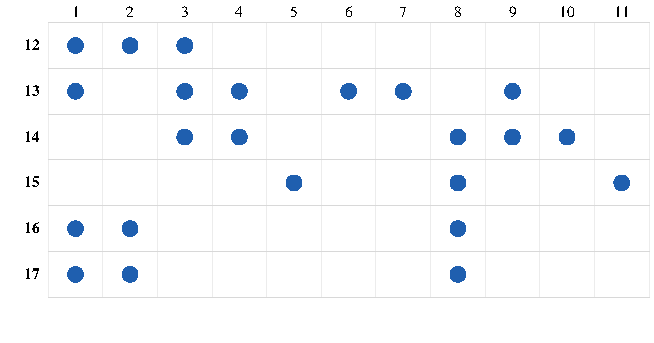
\includegraphics[width=\linewidth]{figures/zaleznosci.pdf}
\sidecaption{Macierz zależności książki. Poziomo --- rozdziały matematyki i narzędzi ($1$--$11$), pionowo --- rozdziały o modelu ($12$--$17$); niebieska kropka oznacza, że rozdział o modelu wymaga danego rozdziału matematyki.
Np.\ blok harmoniczny (rozdz.~13) wymaga alikwotów ($3$), widma i HCQT ($6$, $7$), macierzy ($4$) i konwolucji ($9$); uczenie (rozdz.~15) --- pochodnych ($5$), straty ($8$) i optymalizacji ($11$). \label{rys:mapa}}
\end{figure}

\begin{intuicja}
Gen~6 to nie jeden pomysł, tylko składanka kilku prostych: \emph{logarytm} (żeby wzorzec nuty był niezmienny przy przesunięciu), \emph{widmo} (żeby zobaczyć alikwoty), \emph{konwolucja} (żeby ten sam wzorzec działał wszędzie), \emph{uwaga} (żeby nuty i klatki mogły się nawzajem sprawdzać)
i \emph{entropia krzyżowa z gradientem} (żeby to wszystko dało się nauczyć). Każdy z elementów da się zrozumieć osobno --- i o to chodziło w tej książce.
\end{intuicja}

\section*{Podsumowanie całości}
\begin{itemize}
\item Gen~6: $\mathrm{HCQT}\to$ trzon $\to3\times$ blok harmoniczny $\to$ zejście $\to2\times$ kontekst $\to$ LN $\to5$ głowic; potem dekoder (def.~\ref{def:gen6}).
\item Wymiary się zgadzają (tw.~\ref{tw:wymiary}); największe tablice są wewnątrz bloku harmonicznego (tab.~\ref{tab:ksztalty}).
\item Liczba parametrów: wzór z tw.~\ref{tw:liczba-parametrow}; dla Gen~6 $249\,219$, niezależnie od długości nagrania.
\item Mocne strony: logarytmiczna oś i blok harmoniczny; uwaga między wysokościami i w czasie; maski dostępności etykiet. Ograniczenia: dane syntetyczne, brak ablacji, jedno uruchomienie (rozdział~\ref{rozdz:wyniki}).
\end{itemize}

\begin{sprawdz}
\begin{enumerate}
\item Policz $N$ dla modelu z $H=32$, $D=48$, $W=20$ (pozostałe jak w Gen~6) ze wzoru z tw.~\ref{tw:liczba-parametrow}, rozpisując moduły.
\item Podaj kształty po każdym etapie dla nagrania z $T=100$ klatek.
\item O ile zmieni się $N$, gdyby model obejmował $S=60$ półtonów zamiast $53$ (reszta bez zmian)?
\item Który etap ma największy koszt pamięci aktywacji i ile liczb zajmuje dla $T=243$ (tab.~\ref{tab:ksztalty})? Ile razy więcej niż wejście?
\end{enumerate}
\end{sprawdz}

\subsection*{Rozwiązania}
\begin{enumerate}
\item Trzon: $9\cdot32\cdot21+32=6080$. Blok: $64+7200+192+3104=10\,560$, trzy bloki $31\,680$. Zejście: $32\cdot48\cdot3+48+53\cdot48=4656+2544=7200$. Kontekst: $3\cdot96=288$, TA $9572$, PA $9828$, FF $18\,672$, razem $38\,360$; dwie warstwy $76\,720$. Głowice razem z LN: $12\,563$. Suma $6080+31\,680+7200+76\,720+12\,563=134\,243$.
\item Wejście $[1,9,100,159]$; trzon i bloki $[1,48,100,159]$; zejście $[1,64,100,53]$; kontekst i LN $[1,100,53,64]$; głowice $[1,100,53]$ (cztery) i $[1,100,6,21]$.
\item Zmieniają się tylko osadzenie wysokości ($S\cdot D$: $+7\cdot64=448$) i premie uwagi między wysokościami ($n_h(2S-1)$: z $420$ na $476$, czyli $+56$ w każdej z dwóch warstw, $+112$ razem). Razem $+560$: $N=249\,779$.
\item Wnętrze bloku harmonicznego ($336$ kanałów): $12\,982\,032$ liczb, czyli $37{,}3$ razy więcej niż wejście ($347\,733$).
\end{enumerate}
